% Prof. Dr. Ausberto S. Castro Vera
% UENF - CCT - LCMAT - Curso de Ci\^{e}ncia da Computa\c{c}\~{a}o
% Campos, RJ,  2022
% Disciplina: Paradigma de Desenvolvimento Orientado a Objetos
% Aluno:

\chapterimage{projeto.png} % Table of contents heading image
\chapter{Projeto do Sistema OO}
Este capítulo apresenta a arquitetura do sistema de classes, as interfaces do sistema e as tabelas de dados.

\begin{itemize}


  \item Arquitetura do Sistema que será apresentada neste capítulo mostrará o diagrama de
        componente do sistema completo e de um subsistema específico.
  \item Capturas de tela de todas as interfaces de usuário do sistema
  \item Tabelas de dados que foram utilizadas no sistema.

\end{itemize}

Um projeto orientado a objetos é um processo de criação de um conjunto de modelos de projeto orientados a objetos que são posteriormente usados por programadores para escrever e testar o novo sistema a ser desenvolvido \cite{Satzinger2012}.

\section{Arquitetura do Sistema - Classes}
\begin{itemize}
  \item Arquitetura do sistema completo (Diagrama de Componentes UML)
  \item Arquitetura de um subsistema
  \item Arquitetura de
\end{itemize}



\section{Interfaces do Usu\'{a}rio}
Toda a UI foi desenvolvida pelo autor do trabalho usando Bootstrap, um framework CSS gratuito e de código aberto voltado para desenvolvimento web front-end responsivo e mobile-first. Inclui modelos de design baseados em HTML, CSS e JavaScript para tipografia, formulários, botões, navegação e outros componentes de interface.

\begin{itemize}
  \item \textbf{ Cadastro e Login do Usuário}:
        Um dos requisitos definidos foi que o usuário deve estar cadastrado e logado para acessar o sistema.

        \begin{figure}[H]
          \begin{center}
            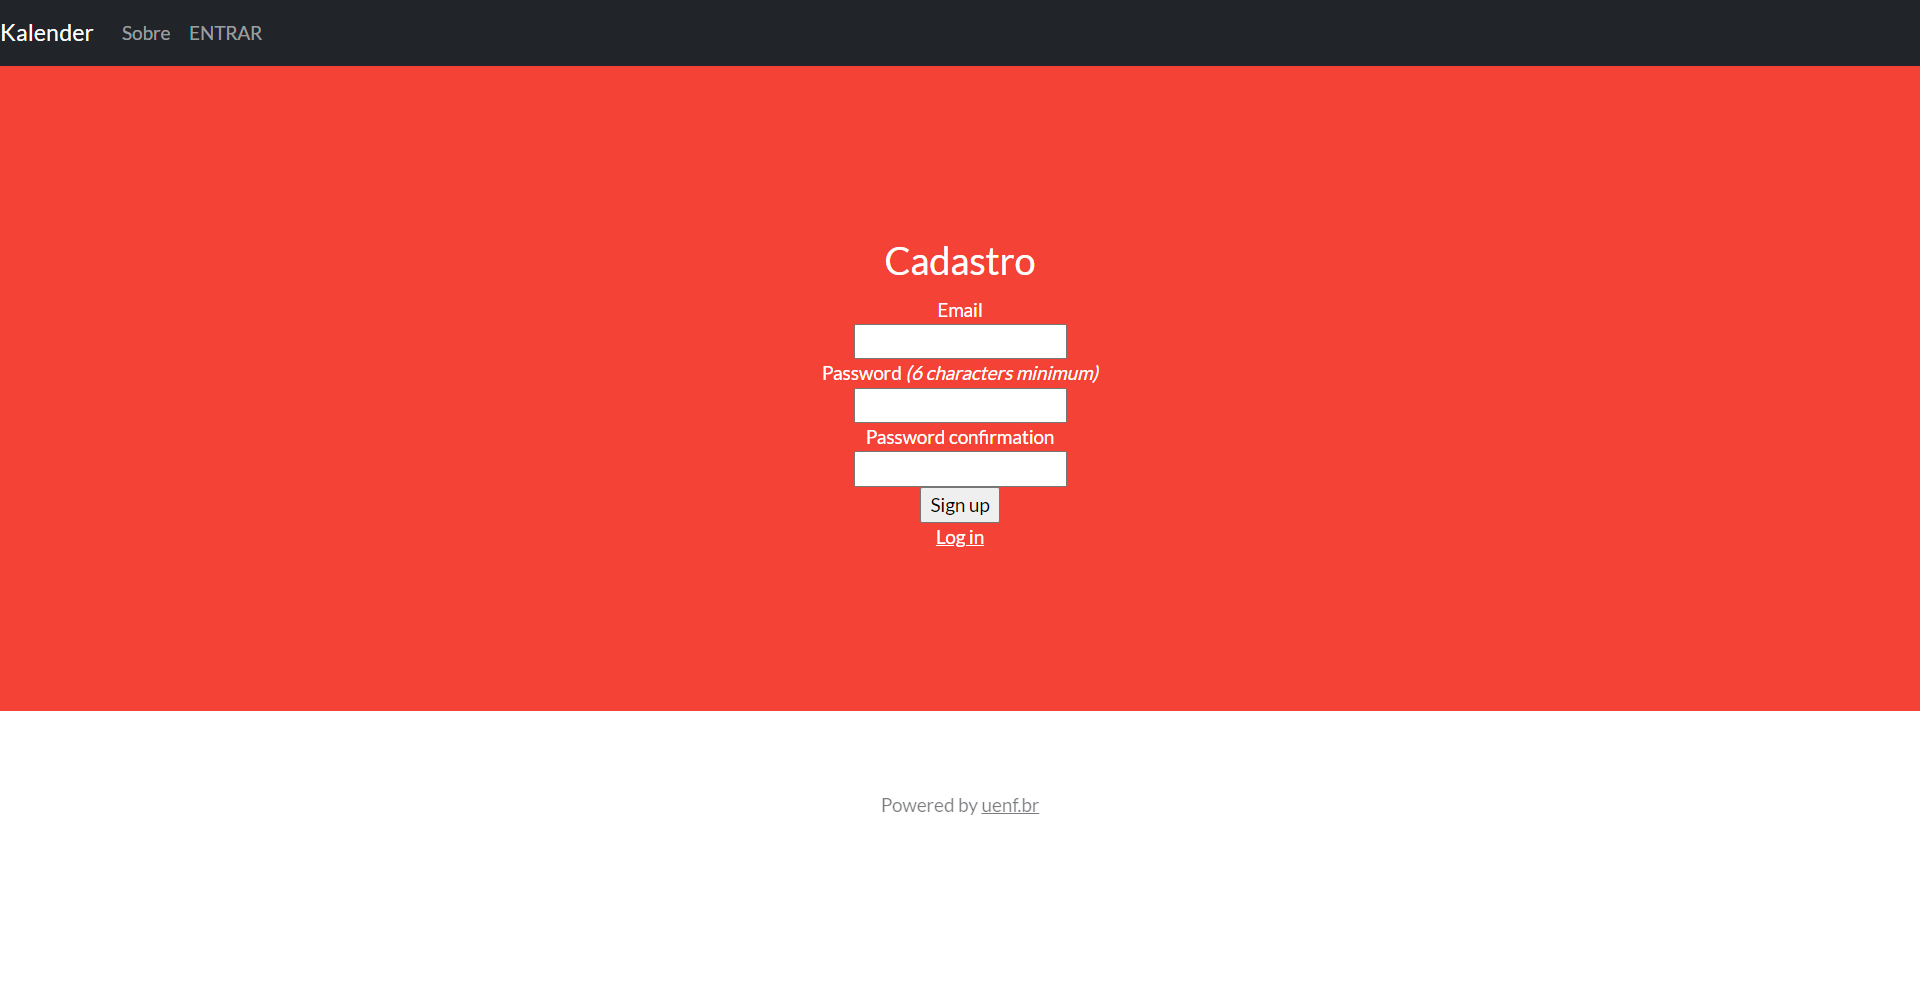
\includegraphics[width=12cm]{Pictures/interface/signup.png}
            \caption{Tela de cadastro de usuário} \label{singup}
          \end{center}
        \end{figure}

        \begin{figure}[H]
          \begin{center}
            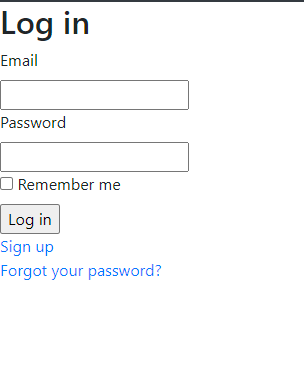
\includegraphics[width=12cm]{Pictures/interface/login.png}
            \caption{Tela de login} \label{login}
          \end{center}
        \end{figure}

  \item \textbf{Recuperação de senha}: Caso o usuário não consiga acessar o sistema será possível solicitar recuperação da senha cadastrada, encontrará a seguinte tela, indicando que o mesmo deve fazer para prosseguir.

        \begin{figure}[H]
          \begin{center}
            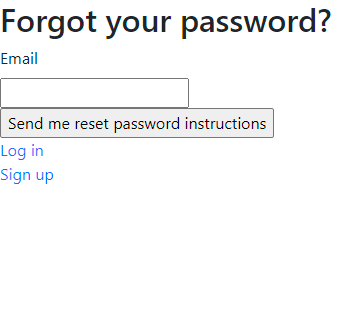
\includegraphics[width=12cm]{Pictures/interface/recuperar.png}
            \caption{Tela de recuperação de senha} \label{recuperar}
          \end{center}
        \end{figure}

  \item \textbf{Home}: Após o login, a página inicial é exibida primeiro. Sua função é apresentar algumas informações relevantes ao usuário.
        \begin{figure}[H]
          \begin{center}
            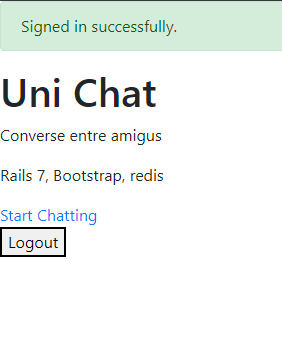
\includegraphics[width=12cm]{Pictures/interface/logged.png}
            \caption{Tela inicial do sistema (home)} \label{recuperar}
          \end{center}
        \end{figure}


              \begin{figure}[H]
                \begin{center}
                  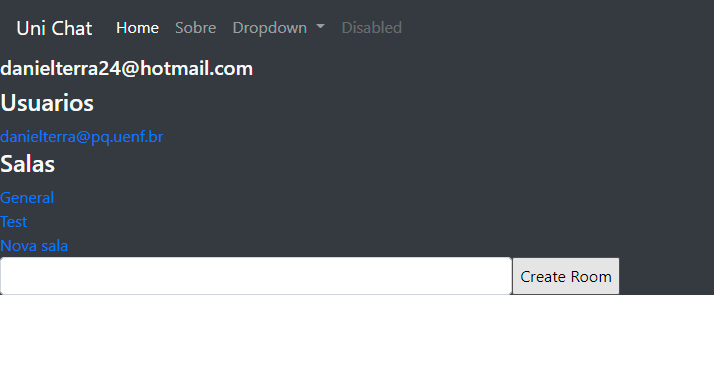
\includegraphics[width=12cm]{Pictures/interface/chat1.png}
                  \caption{Tela inicial (chat)} \label{chat1}
                \end{center}
              \end{figure}
      \end{itemize}


\section{Tabelas de Dados}
Estruturas de dados que fazem parte da base de dados: cada uma com seus atributos e chaves principais e secund\'{a}rias.
